\graphicspath{{design/fig/}}

\chapter{Design}
\section{Design Philosophy}
The aim of this project is to design a impedance spectroscopy system that can be used in a point-of-care setting. Tim Brown's design thinking principles\cite{brownDesignThinking2008} are thus well suited and were used as the bases for the design process. Brown’s approach is characterised by five stages: empathising with the end user, defining a clear problem statement, ideating a wide range of creative ideas, building a quick prototype, and finally testing. These phases are cyclical and allow rapid iteration and learning. This project represents the culmination of this design process, although further iterations of the design process could allow further refinement of the end product.

\subsection{Understanding the end user}
\Ac{POC} diagnostic devices are essential for decentralized healthcare, particularly in resource-limited settings such as rural clinics and community health facilities. While EIS has proven to be a powerful technique for biosensing applications, existing solutions \needscite{present significant barriers to widespread adoption in POC environments.}

Commercial impedance analysers such as the PalmSens4 offer exceptional technical capabilities, including frequency ranges from \SI{10}{\micro\hertz} to 1 MHz, high resolution (18-bit), and data analysis features such as circuit modelling \cite{PalmSens4}. However, these instruments have two critical limitations for \ac{POC} applications. Firstly, they require substantial technical expertise to interpret EIS data, as users must understand the underlying electrochemical principles to extract meaningful diagnostic information. Secondly, commercial systems like the PalmSens4 are prohibitively expensive, with prices \needscite{~\texteuro 15,000}, making them impractical for widespread deployment in clinics, rural health centres, or low-resource settings.

Previous academic projects have successfully demonstrated low cost impedance spectroscopy devices \cite{ebrahimDevelopmentBiosensorEarly2023}\cite{al-aliDesignPortableLowCost2017}\cite{buscagliaSimpleZLowCostPortable2023}, but similarly require users to manually analyse impedance spectra and possess an understanding of EIS principles to interpret the results. This technical barrier prevents POC personnel from using these devices effectively.

\Ac{POC} healthcare providers require a device that performs impedance-based biosensing but abstracts the complexity away from the user, presenting results in an intuitive way. Quantitative results, rather than qualitative results are sufficient to indicate the need for referral to a specialist and further testing. 

\subsection{Problem Statement}

\textbf{How can we design a low-cost, easy-to-use impedance analyzer for biosensing applications that eliminates the need for specialized knowledge, enabling point-of-care personnel to test for multiple biomarkers?}
\newline
This problem statement encapsulates three critical design requirements :
\begin{enumerate}
    \item Accessibility: \needscite{The device must process raw impedance measurements and convert them to meaningful outputs, removing the need for users to understand Nyquist plots, equivalent circuit models, or phase angle analysis. Running from a battery and being able to operate without a computer are also necessities in rural settings.}
    \item Affordability: \rephrase{The total system cost must remain under R4,500 (approximately €220), making it orders of magnitude more affordable than commercial alternatives like the PalmSens4 at €15,000, thereby enabling widespread deployment in resource-limited settings}.
    \item Multiplexing capability: In resource constrained \ac{POC} environments, healthcare professionals often face high patient loads. Due to this, multiplexed \ac{POC} testing is of increasing importance for clinical screening \cite{dincerMultiplexedPointofCareTesting2017}. This allows the screening of multiple analytes with minimal involvement from healthcare professionals.
\end{enumerate}

\section{Functional Design Overview}
The system can be broken up into multiple subsystems, each fulfilling a specific function in order to create a complete device that meets the requirements. On the most basic level the device consists of the \acp{DUT}, an impedance analyser and a user interface. The DUT is the biosensor that interacts with the analyte and whose impedance characteristics change based on the analyte concentration. A multiplexer is used to interface between multiple DUT's and the impedance analyser. The impedance analyser can be further broken down into the \rephrase{power electronics}, excitation stage, voltage and current measurement stages and finally the processing that uses an STM32. The user interface is based on an ESP32 and communicates with the impedance analyser through UART.

\todo{Breek impedance analyser op in further subsystems}
Discuss wat ons wil bereik en hoe ons dit gan opbreek. Beskryf hoe die circuit die beginsels van biosensors en EIS in ag moet neem, basies wat dit moet doen, hoekom multiplexing en ja dan hoe daai overall doel in gedeeltes opgebreek word.

\begin{figure}[H]
    \centering
    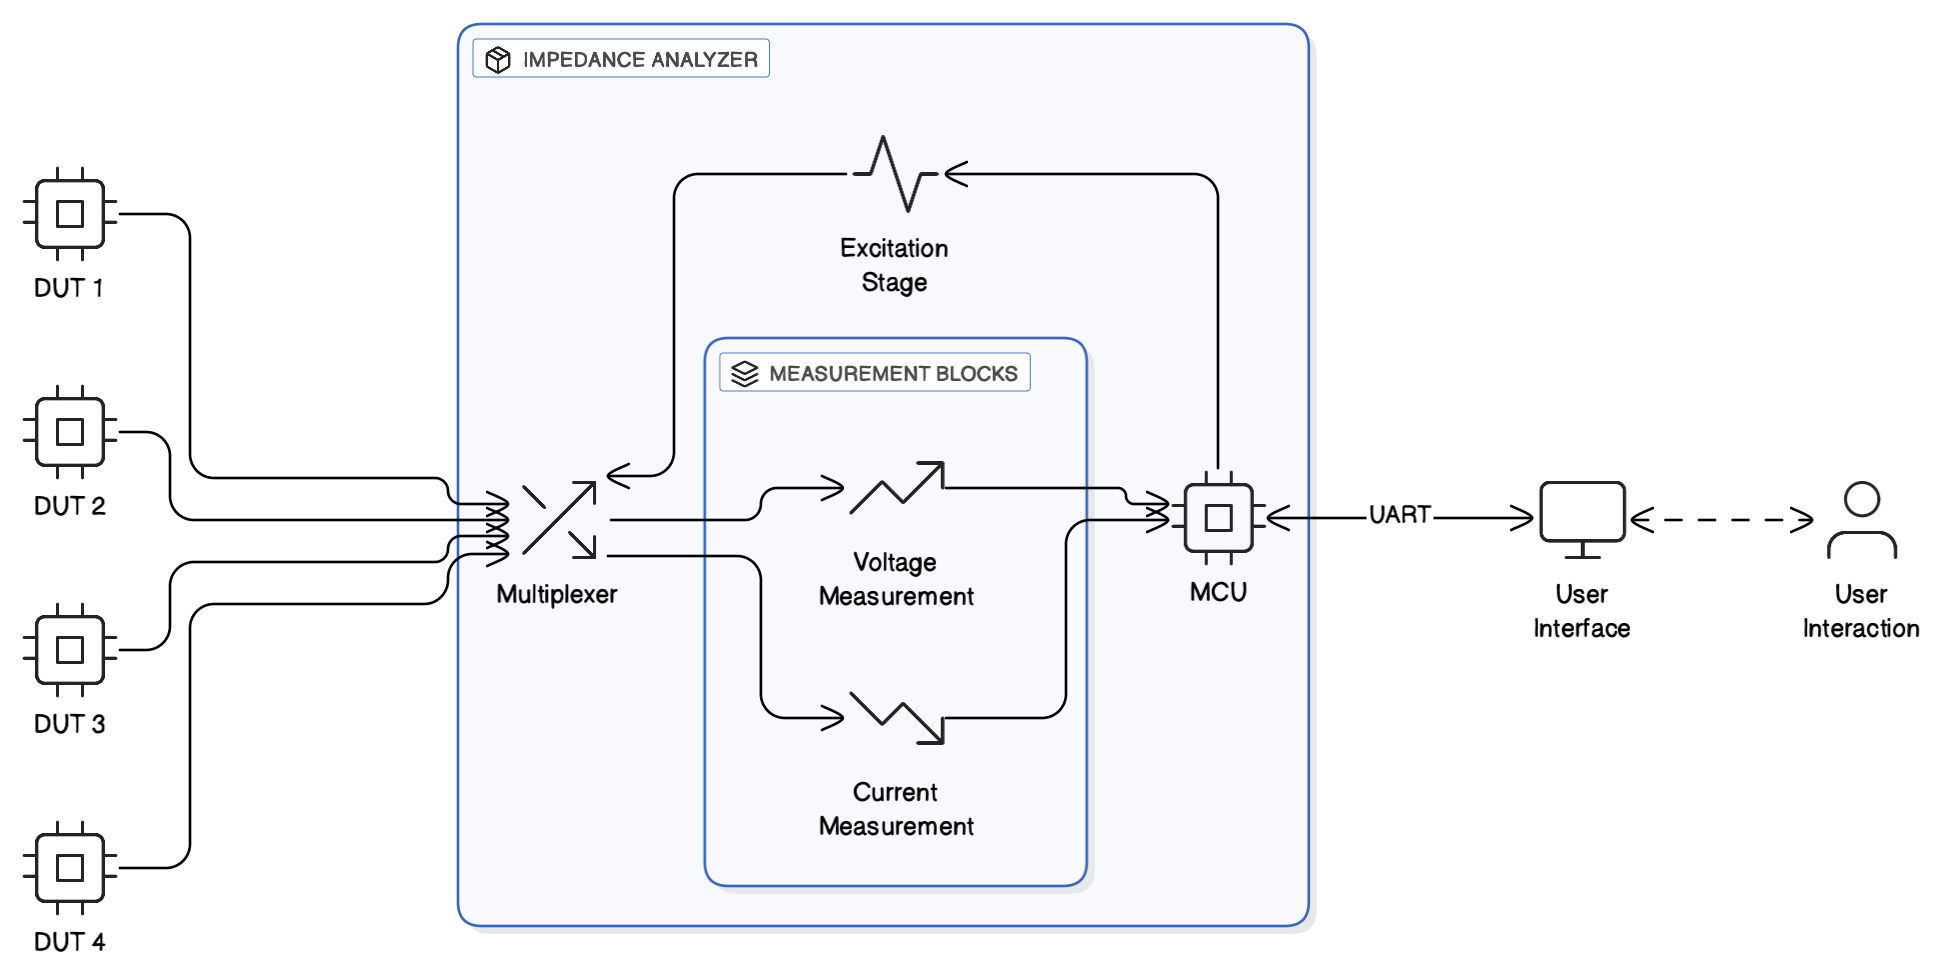
\includegraphics[width=0.8\textwidth]{SystemOverview.png}
    \caption{System Overview}
    \label{fig:system_overview} 
\end{figure}

\section{Subsystem Design}

\subsection{Excitation}\label{subsec:design_excitation}
Discuss opsies vir excitation considered: AD5933 chip wat signals generate, DAC ons MCU ander external DAC. Ultimately DAC op MCU.
Discuss hoekom sein 10mV moet wees en hoekom ons die volle range van die dac moet gebruik (within die linear region).
Finally tie together oor hoekom die excitation phase dus bestaan uit filtering en voltage attenuation
\todo{Should this be in the literature review?}

EIS involves applying a small sinusoidal perturbation to the \ac{DUT} and measuring the response. This can be either a voltage or current signal, \rephrase{while the other is measured}. Generating or measuring voltage is simple as most modern electronics are voltage mode rather than current mode. On the other hand, generating a small current signal is difficult to do accurately and requires circuits such as the improved Howlard current pump. While measuring a current signal also has some complexity, it is significantly easier than generation. It was thus decided that voltage excitation would be used.

\Ac{EIS} relies on the system acting as a linear time-invariant system, but most real-world electrochemical systems are inherently nonlinear \cite{ElectrochemicalMeasurementsElectrochemical}. To approximate linear behaviour and ensure valid results, EIS uses a small AC excitation signal, typically between 1–10 mVpp\cite{EISQualityIndicators}\cite{lazanasErratumElectrochemicalImpedance2025}. At higher amplitudes, the response deviates from ideal sinusoidal form, causing harmonic distortion and invalid measurements. However, making the excitation too small reduces signal-to-noise ratio, so 10 mVpp is commonly used to balance linearity and measurement quality.

The easiest way of producing a controlled voltage signal is using a \ac{DAC}. \fillout{Both dedicated \acp{DAC} and \acp{DAC} built into \acp{MCU} were possible options.} \todo{Figure out hoekom die AD5933 nie sou werk nie (maybe lack of voltage measurement en discuss TIA issues)}

Biosensing requires a bipolar signal with no DC component to avoid charge accumulation at the electrode–electrolyte interface, which leads to polarization. Over time, this would establish a net electrochemical bias, which drives redox reactions and changes the interfacial chemistry of the biosensor. These parasitic reactions alter the impedance characteristics of the electrode, obscuring the true dielectric and charge transfer properties that the EIS measurement aims to quantify. This can be solved by shifting our generated excitation to be biased around ground using a level shifting opamp circuit. However, this also requires providing all analogue circuitry with a negative supply rail. Rather, this project makes use of a buffered virtual ground reference at 1.65V (3.3V/2) and uses this as the midpoint for all the analogue circuitry. This approach ensures that no DC bias is applied to the \ac{DUT} while negating the need for negative supply rails.

When generating a sinusoidal signal using a \ac{DAC}, the output is not a smooth analogue waveform, but rather a series of discrete voltage steps. These steps introduce high-frequency components and harmonics that are not present in the original signal. \trimdown{If these unwanted frequencies are not removed, they can interfere with downstream analogue circuitry or be misinterpreted during subsequent analog-to-digital conversion, a phenomenon known as aliasing.} To prevent this, an anti-aliasing filter (AA filter), typically a \ac{LPF}, is placed after the DAC output to remove high-frequency content and smooth out the signal.

Dynamic range determines the smallest signal the DAC can produce above its noise floor. The theoretical dynamic range (in dB) of a DAC is given by the following formula\cite{gaddyDYNAMICPERFORMANCETESTING}:
\begin{equation}
    \text{Dynamic Range}=6.02n + 1.76 
    \label{eq:dac_range}
\end{equation}
with $n$ being the number of bits of resolution. For the 12-bit \ac{DAC} found in the STM32F303K8, this results in a dynamic range of 74dB. When designing the AA filter, the dynamic range determines the required level of attenuation at the Nyquist frequency ($f_s/2$). To prevent high-frequency components—introduced by the DAC's discrete step output—from being aliased back into the signal band, the AA filter must attenuate these frequencies sufficiently so that any aliased content falls below the DAC's noise floor, as set by its dynamic range. At the same time, the filter's passband must remain flat at the desired signal bandwidth to avoid distorting the amplitude or phase of the intended output. 

\todo{If we want to have more calculations insert, the calcs of how to calculate the cutoff of an 8th order raised cosine to have -74dB at fs/2 but it's going to be at least 1/2 page}

Due to these requirements, a fixed frequency AA filter is unsuitable when generating a wide range of frequencies from 1Hz-100kHz. Many variable AA filter ICs exist, however many require changing a resistor value to set the cutoff frequency. \rephrase{This would be impractical when many frequencies are needed.} Ultimately the LTC1069 proved to be the only viable option, providing an 8th order lowpass filter that approximates a raised cosine response (with $\alpha=1$). Importantly it has a cutoff frequency of up to 120kHz (200kHz when using $\pm5V$ supply rails) set by an external clock and a linear phase response \cite{LTC10697CS8PBF}. \rephrase{The clock-tunable nature of the LTC1069 is ideal for this project, allowing easy adjustments through the use of a timer on the STM.}



\todo{Insert diagrams of stair stepping and frequency components. Dalk sommer van LT Spice}

\subsection{Voltage Measurement}
Some impedance analyser designs attempt to infer voltage across the sample by using the known attenuation an applied signal \cite{buscagliaSimpleZLowCostPortable2023}. However, direct measurement of the true voltage across the device under test ensures all sources of non-ideal behaviour (parasitic resistances, stray capacitance, drift, and environmental changes) are accounted for, providing accurate data for impedance calculation. Accurate voltage monitoring is vital because small changes can significantly affect calculated impedance, particularly in low-voltage biosensing circuits.

It is essential to measure the voltage directly across the biosensor, rather than measuring the applied signal only in reference to the virtual ground. \needscite{This ensures that variations that occur due to the dynamic and non-ideal behaviours at the sensor–electrolyte interface are included, leading to more reliable results.} 

Two common circuits are used to achieve this: differential op-amps and instrumentation amplifiers. Differential op-amps are simple and cost-effective for basic differential measurements, but they are susceptible to common-mode noise and offset errors \cite{technologyWhatAreDrawbacks2024}. Differential op-amps also have low input impedance, which loads the signal source and can affect test results \cite{technologyWhatAreDrawbacks2024}. Instrumentation amplifiers, on the other hand, are specifically designed for high-precision differential measurement and provide superior common-mode rejection, high input impedance and excellent accuracy even when the input signals are small or operating in a noisy environment \cite{InstrumentationAmplifierOperational}. This makes instrumentation amplifiers particularly suitable for biosensing applications where the signals to be measured can be very small, and minimizing interference is critical.

Additionally, it is important to amplify the measured voltage to fully utilise the linear range of the \ac{ADC}, which enhances both sensitivity and resolution. By maximizing the voltage swing within the \ac{ADC}'s input range, the system can discriminate smaller changes in sensor response, thus allowing for better detection of low-concentration analytes.

\subsection{Current Measurement}
The most basic method of measuring current is through making use of a precision shunt resistor. This involves placing a small known resistor in series with the current path and measuring the voltage drop across the resistor. Making use of equation \ref{eq:ohms_law}, the current can be calculated.
\begin{equation}
    V_{drop} = I_{in} \times R_{shunt}
    \label{eq:ohms_law}
\end{equation}
This approach is cheap and easy to implement, but has severe drawbacks. The voltage drop across the resistor impacts the magnitude of the applied perturbation, thereby impacting our measurements. For biosensing, where signal levels are low, even small drops or error sources can affect sensitivity.

Alternatively a \ac{TIA} can be used. A \ac{TIA} makes use of the following properties of op-amps:
\begin{equation}
    V_n \approx V_p
    \label{eq:opamp_V}
\end{equation}
\begin{equation}
    I_n \approx I_p \approx 0
    \label{eq:opamp_I}
\end{equation}
Equation \ref{eq:opamp_V} shows that the positive input (connected to the \ac{DUT}) is driven to the same potential as the negative input (the virtual ground reference at 1.65V), thereby ensuring a low-impedance path for the current. Conversely, equation \ref{eq:opamp_I} means that the TIA has a high input-impedance and that the current from the sensor flows entirely through the feedback resistor. The output voltage is then given by:
\begin{equation}
    V_{out}=I_{in} \times R_{feedback}
    \label{eq:tia_gain}
\end{equation}
The feedback resistor can be large without affecting the applied signal, however it does reduce the bandwidth of the TIA. If $R_{feedback}$ is too large, the TIA will experience significant phase shifts and reduced gain at higher frequencies. This can be mitigated by using multiple gain stages.

Biosensing with a fixed voltage perturbation over a wide impedance range means the current can vary from nanoamps (high impedance, low analyte concentration) to milliamps (high impedance, low analyte concentration). This means that using a fixed gain amplifier is impractical. To achieve accurate measurement across this dynamic range, a \ac{PGA} is used to amplify the TIA output and ensure that the output voltage remains within the optimal range for the \ac{ADC}. The TIA is also designed with multiple gains by switching the feedback resistor values. This prevents saturation for high currents and maximises resolution for low currents.

\subsection{DUT}
The design and manufacture of biosensors are outside the scope of this project. The biosensors described in \cite{ebrahimDevelopmentBiosensorEarly2023} were used for this project, however the system could easily be adapted to work with other capacitive biosensors. To ensure ease-of-use, a method of interfacing with the biosensors that is simple and reliable needed to be developed. Spring loaded battery connectors were used as they allow the DUT to be easily slid in and out of the device when combined with a 3d printed \rephrase{holder}.

\todo{Insert 3d model of connectors, dut and 3d print.}
\subsection{Multiplexer}
Two approaches towards multiplexing were considered. One approach is to have multiple excitation sources and measurement stages, allowing for simultaneous measurements of all \acp{DUT}. \rephrase{This approach has the advantage of speeding up the measurement process, while allowing each \ac{DUT} to have electronics dedicated to its measurement range.} The major disadvantages to this approach is complexity and cost.

Another approach is re-using the same excitation and measurement circuitry, by switching the input and outputs between the \acp{DUT}. This reduces the cost and complexity, but is reliant on having a reliable switching mechanism that does not impact the measurements.

Ultimately the best approach was using a single set of excitation and measurement circuitry, multiplexed in order to measure \acp{DUT} sequentially. The cost reductions of this approach outweighs the increased measurement time as no user input is required between \ac{DUT} measurements.

Various options for multiplexers were considered including dedicated analogue multiplexers (MUX ICs), op-amp based multiplexers and relays. Dedicated analog multiplexers consist of a collection of analog switches. They typically use CMOS technology, resulting in compact integration and fast switching speeds. Modern analogue switches are available with very low on-resistance ($<1\Omega$) and a high degree of flatness \cite{SelectingRightCMOS}. However, leakage currents are inherent to these solid-state devices and can corrupt low-current signals, especially in the nanoampere range \cite{SelectingRightCMOS}. 

Op-amp-based multiplexers such as seen in Figure \ref{fig:opamp_mux} provide buffering and impedance matching, which make them ideal for multiplexing voltage signals, but the buffering also make them unsuitable for use with current signals.

\begin{figure}[H]
    \centering
    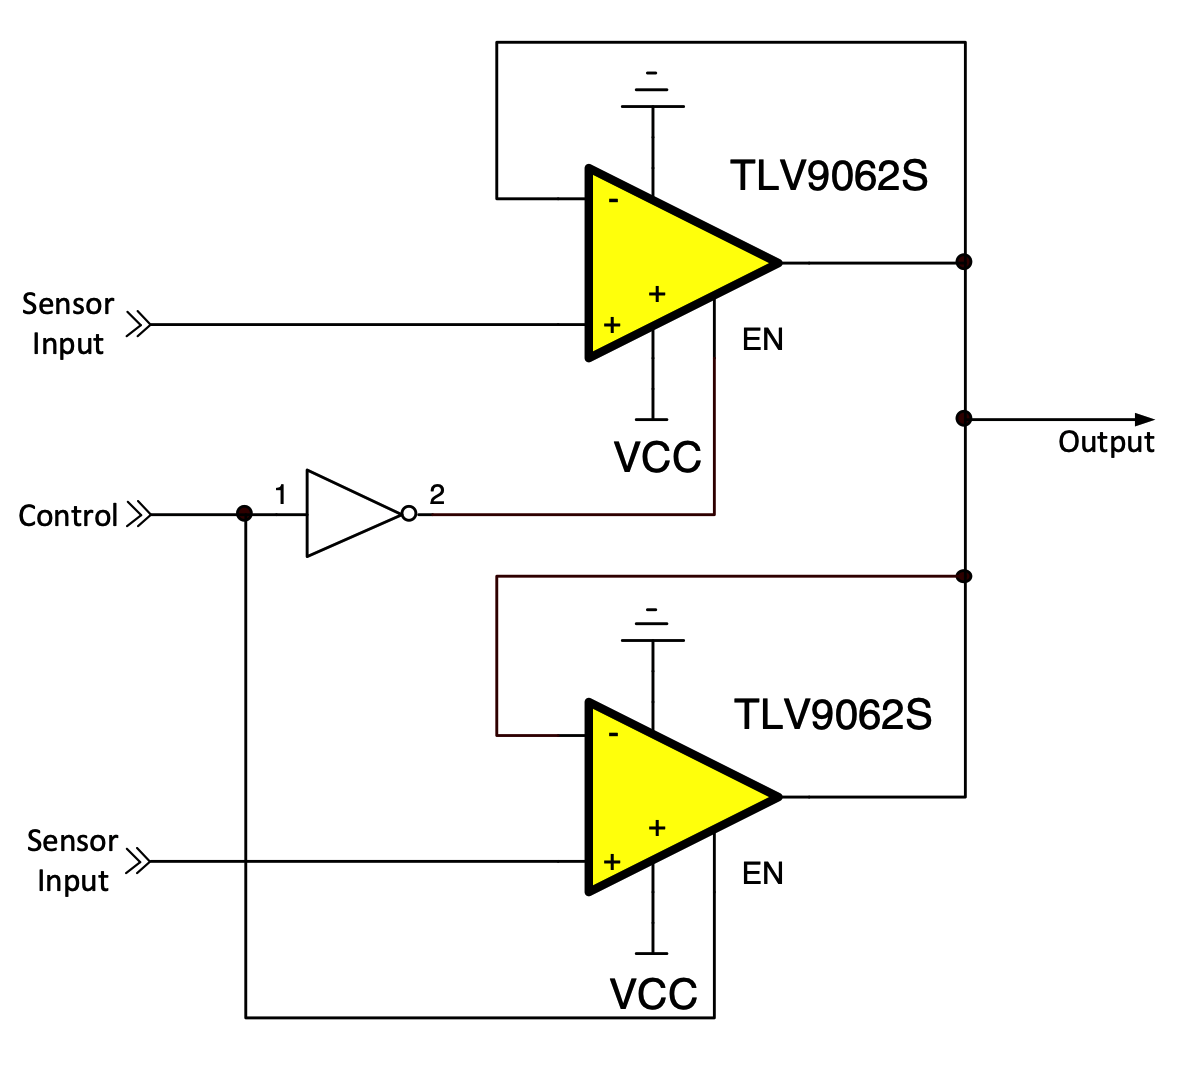
\includegraphics[width=0.4\textwidth]{OpAmpMux.png}
    \caption{Op-amp based multiplexer circuit \cite{Sboa311a}}
    \label{fig:opamp_mux}
\end{figure}

Signal relays, in contrast, use electromechanical contacts to physically open or close signal paths, offering near-zero leakage current and extremely low, stable contact resistance that is independent of signal voltage and temperature. This physical isolation and connection ensures that the measured current accurately reflects the biosensor response. While relays are slower to switch and larger than solid-state alternatives, their switching speed is more than sufficient for switching between sensors.

The TXS2-L2-3V DPDT latching signal relay was chosen due to it's small size, low operating current (23.3 mA) and high mechanical lifetime (Minimum 200 000 operations). The major concern of a mechanical relay is the mechanical wear, however at an assumed 2 actuations per measurement and 50 measurements a day, the relays are expected to last more than 5 years. Utilising the DPDT topology of the relay, they can be configured in a tree pattern, allowing for 4 DUT's to be switched using 3 relays as seen in figure \ref{fig:relay_topology}. 

Despite the low operating current, a driver circuit is still needed to power the relay from a microcontroller GPIO. This consists of a lowside NPN transistor and a flyback diode to protect against voltage spikes when the coil is switched off. The final circuit can be seen in figure \ref{fig:relay_circuit}

\subsection{Power Circuitry}
\rephrase{With portability in mind, a battery is a requirement for the system.} It was decided that the most cost-effective approach would be to utilise a microcontroller with built-in LiPo charging circuitry instead of a dedicated charging circuit as this is commonly available in many ESP32 boards. \rephrase{The 3.3V rail from the ESP will then be used to power the rest of the system.} 

As mentioned in Section \ref{subsec:design_excitation}, a 1.65V reference is needed for the analogue circuitry. Due to the small amplitude of the excitation signal, it needs to be highly accurate and stable. This was done through the use of a matched resistor array and a op-amp buffer. Using a resistor array ensures that our reference is the exact midpoint of the supply voltage despite any tolerances in the precise resistor value, while the op-amp buffers this output to avoid loading the resistor array and causing a voltage drop. Choosing a too large resistor value risks a slightly uneven voltage drop due to the input bias current of the op-amp buffer, on the other hand, a lower value increases the static current draw and power consumption. $1k\Omega$ was chosen as a balance between these tradeoffs.

\begin{figure}[H]
    \centering
    \begin{minipage}{0.35\textwidth}
        \centering
        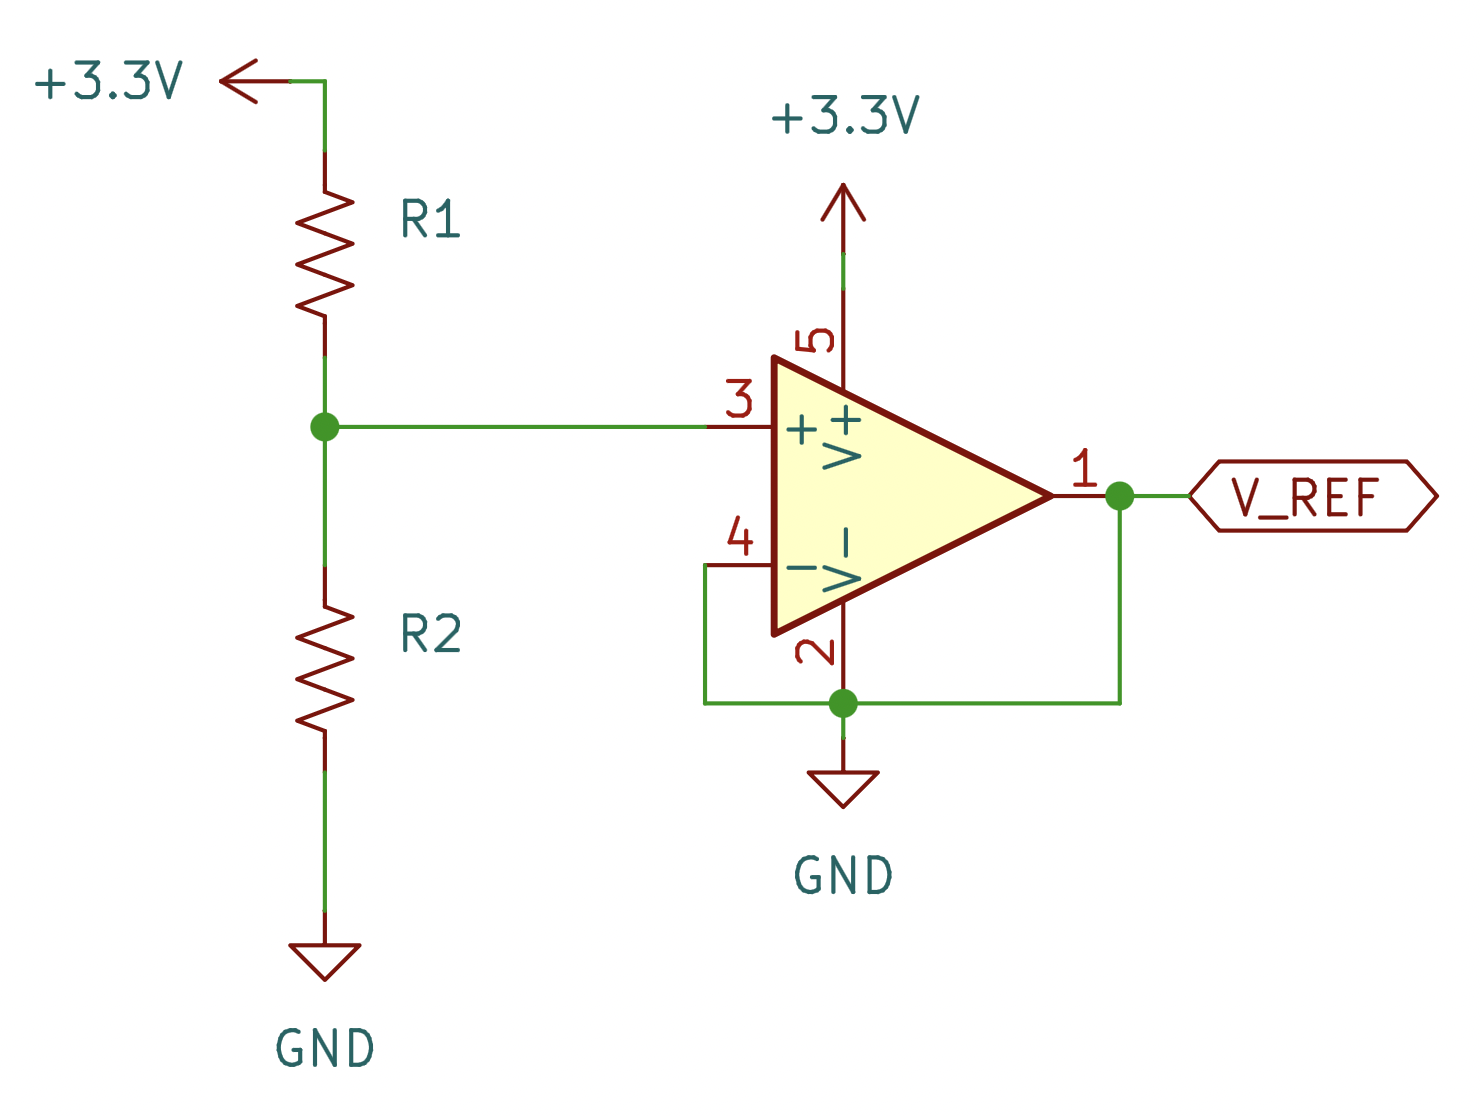
\includegraphics[width=\textwidth]{Vground.png}
        \caption{\newline Virtual ground reference circuit}
        \label{fig:virtual_ground}
    \end{minipage}\hfill
    \begin{minipage}{0.6\textwidth}
        \centering
        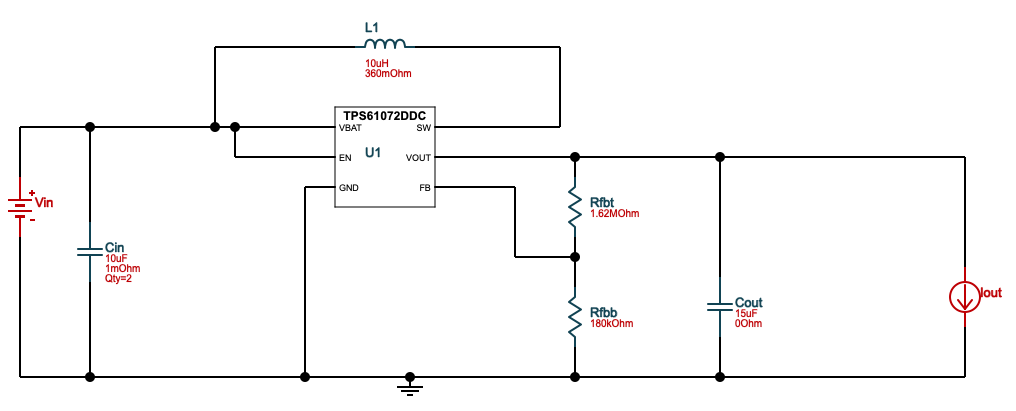
\includegraphics[width=\textwidth]{5V_Reg.png}
        \caption{5V boost converter circuit}
        \label{fig:5V_reg}
    \end{minipage}
\end{figure}

The LTC1069 AA-Filter requires a 5V supply voltage. A 3.3V to 5V boost circuit was designed around the TPS61072 boost regulator using the TI WeBench power supply design tool \cite{WEBENCHCIRCUITDESIGNERDesignTool}, ensuring a stable and efficient circuit as seen in figure \ref{fig:5V_reg}. 

\subsection{Signal Processing}

\subsection{User Interface}
\todo{Fill in once GUI is actually done}
\todo{Talk about flexibility of having both physical buttons and display aswell as web ui, allowing both standalone use and use with either computer, tablet or cell phone, ensuring versatility across environments}

\section{Detailed Design}
Gaan meer in diepte oor circuitry maar steeds met generic/ideal coponents. Cover circuitry van elke section, design requirements etc soos 10mV excitation bv. Wat wil ons bereik en dan hoe daai translate na technical requirements en dan die circuitry. Wys LT Spice circuits en sims van elke seksie en combined. Cost is n spec (<R4500). Refer back to Brown design. Noem dat weens die tight budget and time restrictions van die projek was prototyping gedoen met SPICE en bullshit iets van basiese toetse met esp's en stm's wat rondlê maar anders is as finaal?

\subsection{DUT}
Data van Dr Ebrahim, en dan kry circuit model van daai af.

\subsection{Voltage Reference}
DONE

\subsection{Excitation Stage}
Verduidelik hoekom ons 3.3V output signal van DAC gebruik (maximise range theory). Verduidelik hoekom ons 10mV soek gebasseer op DUT circuit model. Gee brief overview van beginsels van opamp em somme. Verduidelik dan hoekom LPF Anti Aliasing nodig is gebasseer op Frequency domain theory en al daai. Calcs rondom hoe naby aan signal freq cutoff moet wees, dus variable LPF. Te expenny om self te bou dus eerder IC. Was voor en na Filter van DAC sims.

\subsection{Voltage Measurement}
Why is voltage measurement needed when we already know our output voltage. Discuss what to consider when amplifying signal. Discuss LPF en hoekom n volle variable een nie needed is nie (dit is meestal vir noise nie vir anti aliasing van sampling nie, want DAC AA behoort dit te keer).

\subsection{Current Measurement}
Beskryf hoekom current measurement so belangrik is. Wat ons range van currents is. Beskryf beginsels van TIA including somme en circuit analysis. Dan hoekom TIA nie al die amplifications doen nie en why PGA needed is. Raak dan briefly ook op die LPF beginsel selfde as voltage.

\subsection{Multiplexing}
DONE

\subsection{DSP}
Discuss why DSP needed, why microcontroller and not other DSP. Beskryf basies hoe ons filtering gaan doen etc. Die formules en konsepte van freq domain en hoe ons capacitance calc en dan na concentration gaan. Los die details van code en libraries en issues vir Firmware Design section.

\subsection{User Interface}
Baie briefly discuss wat ons vereis van

\section{Component Selection}
Watse komponente ons kies, why en watse aspekte ons consider het en hoekom daai specs belangrik is. How een komponent die ander beinvloed. Wys sims met spesifieke komponent seleksies. Wys calcs vir passive compoinent selections.

\section{PCB Design}
Beskryf filosofie en idees wat mee ingegaa het. Briefly discuss general PCB design principles wat design geguide het (Analogue ground plane etc). Beskryf beperkings van PCB manufactures wat inag geneem moes word (PCB size, layers, trace width via diamtre etc.). Noem briefly hoekom PCB in China eerder as Uni laat maak. Gaan deur design logic en discuss probleem met TIA. Include maybe final PCB diagram en langs dit foto van manufactured PCB.

\section{Firmware Design}
Inculde flow diagram.

\subsection{ESP}
Vertel van wat ons wil bereik en hoekom. Discuss libraries used. Discuss maybe issues rondom C6 en hoe dit gesolve is en hoekom die C6 steeds die rgete keuse was.

\subsection{STM}
Probleme met arm library te groot. Discuss met flow chart hoe DMA en als met DAC en ADC interact en dan UART en badies program flow. Delve into limits van STM en maybe briefly setup van DAC en ADC.

\label{chap:design}